%%%%%%%%%%%%%%%%%%%%%%%%%%%%%%%%%%%%%%%%%
% Beamer Presentation
% LaTeX Template
% Version 1.0 (10/11/12)
%
% This template has been downloaded from:
% http://www.LaTeXTemplates.com
%
% License:
% CC BY-NC-SA 3.0 (http://creativecommons.org/licenses/by-nc-sa/3.0/)
%
%%%%%%%%%%%%%%%%%%%%%%%%%%%%%%%%%%%%%%%%%

%----------------------------------------------------------------------------------------
%	PACKAGES AND THEMES
%----------------------------------------------------------------------------------------

\documentclass[10pt]{beamer}

\mode<presentation> {

% The Beamer class comes with a number of default slide themes
% which change the colors and layouts of slides. Below this is a list
% of all the themes, uncomment each in turn to see what they look like.

%\usetheme{default}
%\usetheme{AnnArbor}
%\usetheme{Antibes}
%\usetheme{Bergen}
%\usetheme{Berkeley}
%\usetheme{Berlin}
%\usetheme{Boadilla}
%\usetheme{CambridgeUS}
%\usetheme{Copenhagen}
%\usetheme{Darmstadt}
%\usetheme{Dresden}
%\usetheme{Frankfurt}
%\usetheme{Goettingen}
%\usetheme{Hannover}
%\usetheme{Ilmenau}
%\usetheme{JuanLesPins}
%\usetheme{Luebeck}
\usetheme{Madrid}
%\usetheme{Malmoe}
%\usetheme{Marburg}
%\usetheme{Montpellier}
%\usetheme{PaloAlto}
%\usetheme{Pittsburgh}
%\usetheme{Rochester}
%\usetheme{Singapore}
%\usetheme{Szeged}
%\usetheme{Warsaw}

% As well as themes, the Beamer class has a number of color themes
% for any slide theme. Uncomment each of these in turn to see how it
% changes the colors of your current slide theme.

%\usecolortheme{albatross}
%\usecolortheme{beaver}
%\usecolortheme{beetle}
%\usecolortheme{crane}
%\usecolortheme{dolphin}
%\usecolortheme{dove}
%\usecolortheme{fly}
%\usecolortheme{lily}
%\usecolortheme{orchid}
%\usecolortheme{rose}
%\usecolortheme{seagull}
%\usecolortheme{seahorse}
%\usecolortheme{whale}
%\usecolortheme{wolverine}

%\setbeamertemplate{footline} % To remove the footer line in all slides uncomment this line
%\setbeamertemplate{footline}[page number] % To replace the footer line in all slides with a simple slide count uncomment this line

\setbeamertemplate{navigation symbols}{} % To remove the navigation symbols from the bottom of all slides uncomment this line
}

\usepackage{graphicx} % Allows including images
\usepackage{booktabs} % Allows the use of \toprule, \midrule and \bottomrule in tables
\usepackage{hyperref}
\usepackage{tikz}
\usepackage{algpseudocode}
\setbeamerfont{frametitle}{size=\large}
\setbeamerfont{framesubtitle}{size=\small}

%----------------------------------------------------------------------------------------
%	TITLE PAGE
%----------------------------------------------------------------------------------------

\title[Cooperative Explorer]{COEX-1} % The short title appears at the bottom of every slide, the full title is only on the title page
\subtitle{Cooperative Explorer}
\author[Aurélien Werenne]{Aurélien Werenne \\ {\small Advisor: Prof. B. Boigelot}} 
\institute[ULiège] 
{
University of Liège \\ 
\medskip
Link to code: \href{https://github.com/Werenne/multi-agent-mapping}{\textcolor{blue}{Github}}

}
\date{\today} 

\begin{document}

\begin{frame}
\titlepage 
\end{frame}

\begin{frame}
\frametitle{Overview} 
\tableofcontents 
\end{frame}

%----------------------------------------------------------------------------------------
%	PRESENTATION SLIDES
%----------------------------------------------------------------------------------------

%------------------------------------------------
\section{General} 
%------------------------------------------------

\begin{frame}
\frametitle{Overview}
\tableofcontents[currentsection,subsectionstyle=shaded]
\end{frame}

%------------------------------------------------
\begin{frame}
\frametitle{General}
\framesubtitle{Objective}
The goal of the robot, named COEX-1, is to map an unknown environment in a centralized multi-agent setting.\\~\\
The main features of the robot are:
\begin{itemize}
\item Following a black line
\item Computing the travelled distance
\item Detecting, classifying and handling intersections
\item Avoiding obstacles
\item Communicating with a central unit 
\end{itemize}
\end{frame}

%------------------------------------------------
\begin{frame}
\frametitle{General}
\framesubtitle{Material}
Non-exhaustive list of used components:
\begin{itemize}
\item Microcontroller (Arduino Nano) 
\item Reflectance sensor array (Pololu QTR-MD-06A)
\item Digital distance sensor (Sharp GP2Y)
\item Magnetic encoders 
\item DC Motor (Pololu 150:1 micro metal gearmotor MP)
\item Motor driver (L298N dual H-bridge) 
\item Battery (NiMH 7.2V) 
\item Bluetooth module (HC-05) 
\end{itemize}
\end{frame}

%------------------------------------------------

\begin{frame}
\frametitle{General}
\framesubtitle{Structure (1/3)}
\begin{figure}[hbtp]
\centering
\begin{tikzpicture}
	\node [anchor=west] (bluetooth) at (-1.6,5) {\small Bluetooth};
	\node [anchor=west] (nano) at (-1.6,3) {\small Nano};
	\node [anchor=west] (sharp) at (-1.6,1) {\small Sharp};
	\node[anchor=south west,inner sep=0] (image) at (0,0) {\includegraphics[scale=0.05]{figures/img_front.JPG}};
	\begin{scope}[x={(image.south east)},y={(image.north west)}]
		%\draw[help lines,xstep=.1,ystep=.1] (0,0) grid (1,1);
		\draw[yellow,ultra thick,rounded corners] (0.62,0.25) rectangle (0.72,0.40);
		\draw[yellow,ultra thick,rounded corners] (0.35,0.60) rectangle (0.45,0.83);
		\draw[yellow,ultra thick,rounded corners, rotate around={48:(0.55,0.50)}] (0.55,0.50) rectangle (0.65,0.70);
		\draw [-latex, ultra thick, yellow] (bluetooth) to[out=0, in=-120] (0.35,0.6);
		\draw [-latex, ultra thick, yellow] (nano) to[out=0, in=-120] (0.5,0.55);
		\draw [-latex, ultra thick, yellow] (sharp) to[out=0, in=-160] (0.62,0.32);
	\end{scope}
\end{tikzpicture}
\caption{Front view of COEX-1}
\end{figure}
%
\end{frame}

%------------------------------------------------

\begin{frame}
\frametitle{General}
\framesubtitle{Structure (2/3)}
\begin{figure}[hbtp]
\centering
\label{fig:fig-img-side}
\begin{tikzpicture}
	\node [anchor=west] (battery) at (-1.6,5) {\small Battery};
	\node [anchor=west] (shield) at (-1.6,3) {\small Shield};
	\node[anchor=south west,inner sep=0] (image) at (0,0) {\includegraphics[scale=0.05]{figures/img_side.JPG}};
	\begin{scope}[x={(image.south east)},y={(image.north west)}]
		%\draw[help lines,xstep=.1,ystep=.1] (0,0) grid (1,1);
		\draw[yellow,ultra thick,rounded corners] (0.65,0.35) rectangle (0.75,0.62);
		\draw[yellow,ultra thick,rounded corners] (0.38,0.23) rectangle (0.55,0.35);
		\draw [-latex, ultra thick, yellow] (battery) to[out=0, in=120] (0.65,0.62);
		\draw [-latex, ultra thick, yellow] (shield) to[out=0, in=-120] (0.38,0.23);
	\end{scope}
\end{tikzpicture}
\caption{Side view of COEX-1}
\end{figure}
\end{frame}

%------------------------------------------------

\begin{frame}
\frametitle{General}
\framesubtitle{Structure (3/3)}
\begin{figure}[hbtp]
\centering
\label{fig:fig-img-bottom}
\begin{tikzpicture}
	\node [anchor=west] (array) at (-2.6,5) {\small Reflectance array};
	\node [anchor=west] (motors) at (-1.6,3) {\small Motors};
	\node[anchor=south west,inner sep=0] (image) at (0,0) {\includegraphics[scale=0.048]{figures/img_bottom.JPG}};
	\begin{scope}[x={(image.south east)},y={(image.north west)}]
		%\draw[help lines,xstep=.1,ystep=.1] (0,0) grid (1,1);
		\draw[yellow,ultra thick,rounded corners] (0.47,0.5) rectangle (0.68,0.65);
		\draw[yellow,ultra thick,rounded corners] (0.38,0.11) rectangle (0.75,0.25);
		\draw [-latex, ultra thick, yellow] (array) to[out=0, in=120] (0.47,0.65);
		\draw [-latex, ultra thick, yellow] (motors) to[out=0, in=150] (0.55,0.25);
	\end{scope}

\end{tikzpicture}
\caption{Bottom view of COEX-1}
\end{figure}
\end{frame}

%------------------------------------------------

\begin{frame}
\frametitle{General}
\framesubtitle{Nomenclature}
Let us explain some notions:
\begin{itemize}
\item error line: ...
\item target speed: ...
\item progress speed: ...
\item measured speed: ...
\end{itemize}
\end{frame}

%------------------------------------------------
\section{Components} 
%------------------------------------------------

\begin{frame}
\frametitle{Overview}
\tableofcontents[currentsection,subsectionstyle=shaded]
\end{frame}

%------------------------------------------------
\begin{frame}
\frametitle{Components}
\framesubtitle{Sharp sensor}
Clean, no noise. Note we had to use bypass capacitor. Threshold at 2 volt, lower than middle because it is preferred to have False Positive than False Negatives.
\begin{figure}[hbtp]
\centering
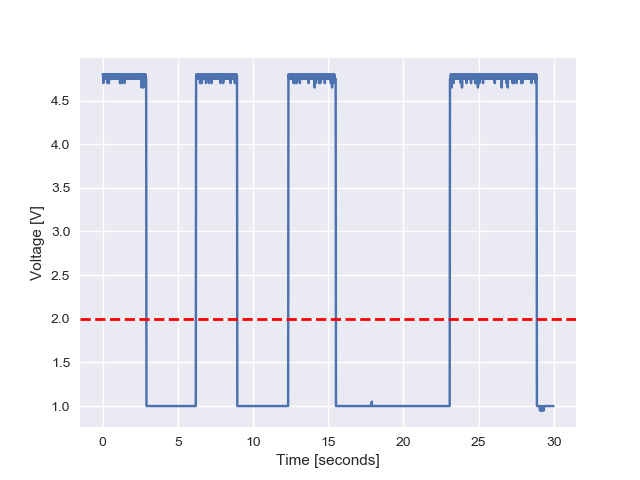
\includegraphics[scale=0.45]{figures/sharp-flow.png}
\caption{Back and forth movement of obstacle going in and out of reach of the sensor}
\end{figure}
\end{frame}


%------------------------------------------------

\begin{frame}
\frametitle{Components}
\framesubtitle{Reflectance sensor array (line sensor)}
Experimentally, we found it is best to average four reading at 100 Hz. On Fig.\ref{fig:flow-qtr} we can see the detection varies smoothly as desired.
\begin{figure}[hbtp]
\centering
\label{fig:flow-qtr}
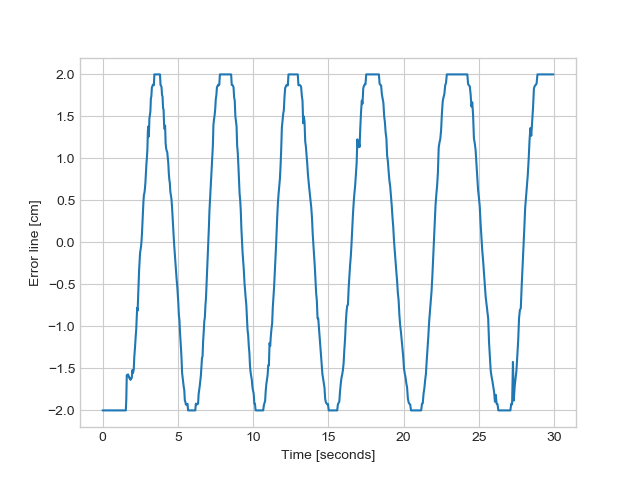
\includegraphics[scale=0.45]{figures/qtr-flow.png}
\caption{Moving black line back and forth between left and right side of the sensor}
\end{figure}
\end{frame}

%------------------------------------------------

\begin{frame}
\frametitle{Components}
\framesubtitle{Shield}
In order for the robot to being able of climbing hills, the line sensors are fixed vertically well above the recommendations of the manufacturer. \\~\\
This decision made the reflectance sensor particularly sensitive to ambient light interferences. As a solution a shield was constructed. 
\end{frame}

%------------------------------------------------

\begin{frame}
\frametitle{Components}
\framesubtitle{Bluetooth module (1/5)}
Sinus test with diagram. Why sinus, fitting etc. Conclusion.
\end{frame}

%------------------------------------------------

\begin{frame}
\frametitle{Components}
\framesubtitle{Bluetooth module (2/5)}
\begin{figure}[hbtp]
\centering
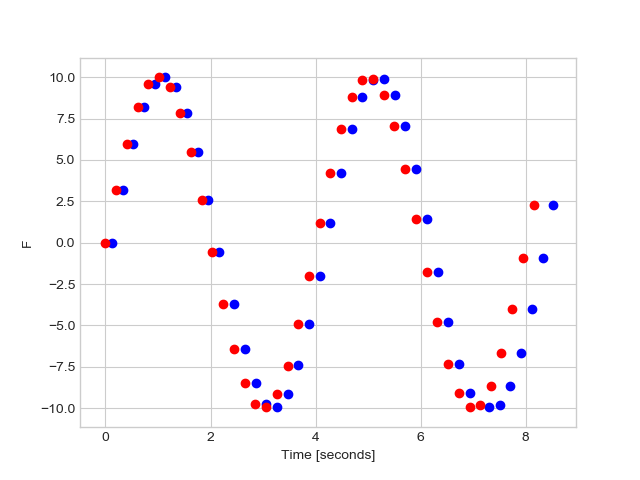
\includegraphics[scale=0.45]{figures/sin-sending-merged-5hz.png}
\caption{Sinus test at 5Hz}
\end{figure}
\end{frame}

%------------------------------------------------

\begin{frame}
\frametitle{Components}
\framesubtitle{Bluetooth module (3/5)}
Explain sender-receiver distortion.Conclusion.
\begin{figure}[hbtp]
\centering
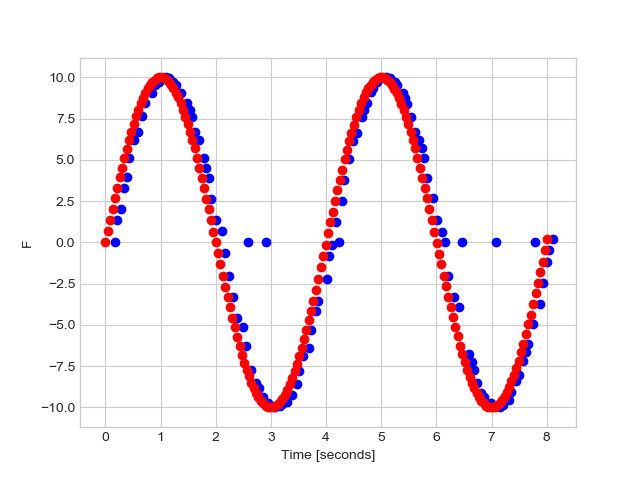
\includegraphics[scale=0.45]{figures/sin-sending-merged-25hz.png}
\caption{Sinus test at 25Hz}
\end{figure}

\end{frame}

%------------------------------------------------

\begin{frame}
\frametitle{Components}
\framesubtitle{Bluetooth module (4/5)}
Explain sender-receiver distortion.Conclusion.
\begin{figure}[hbtp]
\centering
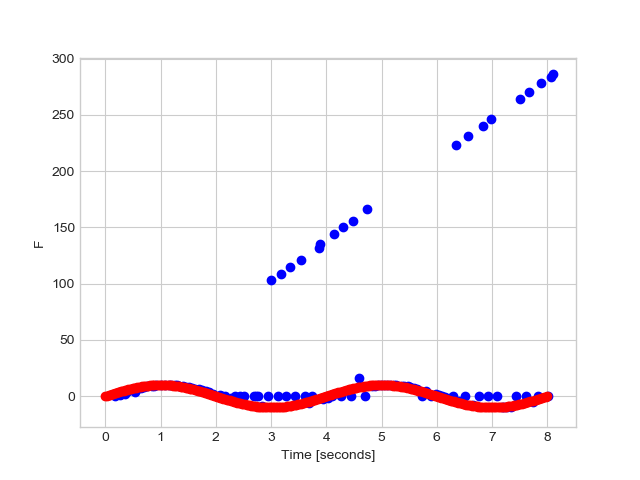
\includegraphics[scale=0.45]{figures/sin-sending-merged-40hz.png}
\caption{Sinus test at 40Hz}
\end{figure}

\end{frame}
%------------------------------------------------

\begin{frame}
\frametitle{Components}
\framesubtitle{Bluetooth module (5/5)}
A voltage divider was used because of the difference in logic level voltage between the Arduino ($0-5$ Volt) and the bleutooth module ($0-3.3$ Volt). 
\begin{columns}[c]

\column{.35\textwidth}
\begin{align*} 
V_{arduino} &=  \frac{R_2}{R_1+R_2}V_{bleutooth} \\[0.4cm]
 &=  \frac{2.2}{3.2}V_{bleutooth}
\end{align*}

\column{.65\textwidth}
\begin{figure}[hbtp]
\centering
\includegraphics[scale=0.07]{figures/diag-voltage-divider}
\caption{Voltage divider}
\end{figure}

\end{columns}
\end{frame}

%------------------------------------------------

\begin{frame}
\frametitle{Components}
\framesubtitle{Quadrature encoders (1/2)}
Magnetic quad encoders using Hall effect to count the number of revolutions of the motor shaft: $n_L$ and $n_R$. The angular velocity of the wheel is computed as follows:
$$ 
w_L = 2\pi f_L
\qquad\text{with}\qquad	
f_L = \frac{n_L}{N' \, G_b \, \Delta{t} }
$$
with $N'$ the number of counts per revolution per channel, and $G_b$ the gearbox ratio. The robot can be modelled as a differential steering wheel such that,
$$ 
v = \frac{v_L + v_R}{2} = \frac{R(w_L + w_R)}{2}
$$
\end{frame}

%------------------------------------------------

\begin{frame}
\frametitle{Components}
\framesubtitle{Motors}
On Fig.\ref{fig:pwm-speed} we observe small differences between left and right motor and it even depends on the charge. To obtain a robust robot, a regulated system need to be designed.
\begin{figure}[hbtp]
\centering
\label{fig:pwm-speed}
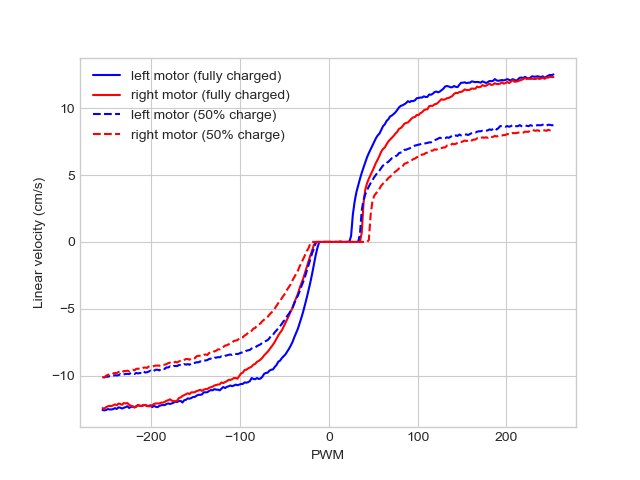
\includegraphics[scale=0.45]{figures/motors_merged.png}
\caption{Relationship between PWM (input) and measured speed (output)}
\end{figure}
\end{frame}


%------------------------------------------------
\section{Control} 
%------------------------------------------------

\begin{frame}
\frametitle{Overview}
\tableofcontents[currentsection,subsectionstyle=shaded]
\end{frame}

%------------------------------------------------
\begin{frame}
\frametitle{Control}
\framesubtitle{General framework (1/2)}
An auto-regulated system is acheived by using several PID controllers. The output of a PID controller can be expressed as
$$ 
o_n (e_n;e_1...e_{n-1}) \leftarrow K_p e_n + K_d\frac{e_n - e_{n-1}}{\Delta t_{n-1:n}} + K_e\sum_{i=0}^{n}{e_i \Delta t_{n-1:n}}
$$
with the following two precautions: anti-windup and anti-derivative kick:
$$
o_n = \left\{
    \begin{array}{ll}
        max & \mbox{if } o_n > max \\
        min & \mbox{if } o_n < min \\
        o_n & \mbox{otherwise.}
    \end{array}
\right.
\qquad\text{and}\qquad	
K_d = \left\{
    \begin{array}{ll}
        0 & \mbox{if } n < T \\
       K_d & \mbox{otherwise.}
    \end{array}
\right.
$$
\end{frame}

%------------------------------------------------

\begin{frame}
\frametitle{Control}
\framesubtitle{General framework (2/2)}
The three main controllers are used to control the speed, direction and aligning when turning (more explanations further).\\~\\
The pwm value is computed from the three controllers outputs:
$$ 
\left\{
    \begin{array}{ll}
		\alpha = o(e_{direction}) \\[0.3cm]
		\beta = o(e_{speed}) \\[0.3cm]
		\gamma = o(e_{align})
	\end{array}
\right.
\Rightarrow
\left\{
    \begin{array}{ll}
		{pwm}_L =  (\beta -\gamma) + \alpha \\
		{pwm}_R = (\beta - \gamma) - \alpha
	\end{array}
\right.
$$
\end{frame}

%------------------------------------------------

\begin{frame}
\frametitle{Control}
\framesubtitle{Direction control (1/2)}
We define three type of desired direction behaviours:
\begin{itemize}
\item \textit{forward}: going in straight direction, setpoint value put such that $v_L = v_R \Rightarrow e_{direction} = v_R - v_L$
\item \textit{line-following}: adapt direction in order that line always centered, $e_{direction} = err_{line}$
\item \textit{turning}: to obtain pure rotation, the following constraint must be satisfied, $v_L = -v_R \Rightarrow e_{direction} = v_L + v_R$ 
\end{itemize}
\end{frame}

%------------------------------------------------

\begin{frame}
\frametitle{Control}
\framesubtitle{Direction control (2/2)}
On Fig.\ref{fig:flow-qtr}, different trajectories of line-following on a straight line with initial disalignment are plotted.
\end{frame}

%------------------------------------------------

\begin{frame}
\frametitle{Control}
\framesubtitle{Speed control (1/5)}
The error in speed control ($e_{speed}$) is the difference between progress and measured speed. For a uniform acceleration as in Fig.\ref{fig:uniform-acc}, the progress speed is computed as follows. 
$$
v_{n+1} \leftarrow v_n + A \, \Delta t_{n:n+1}
\qquad\text{with}\qquad
A = \frac{v_{target}}{T}
$$
\begin{figure}[hbtp]
\centering
\label{fig:uniform-acc}
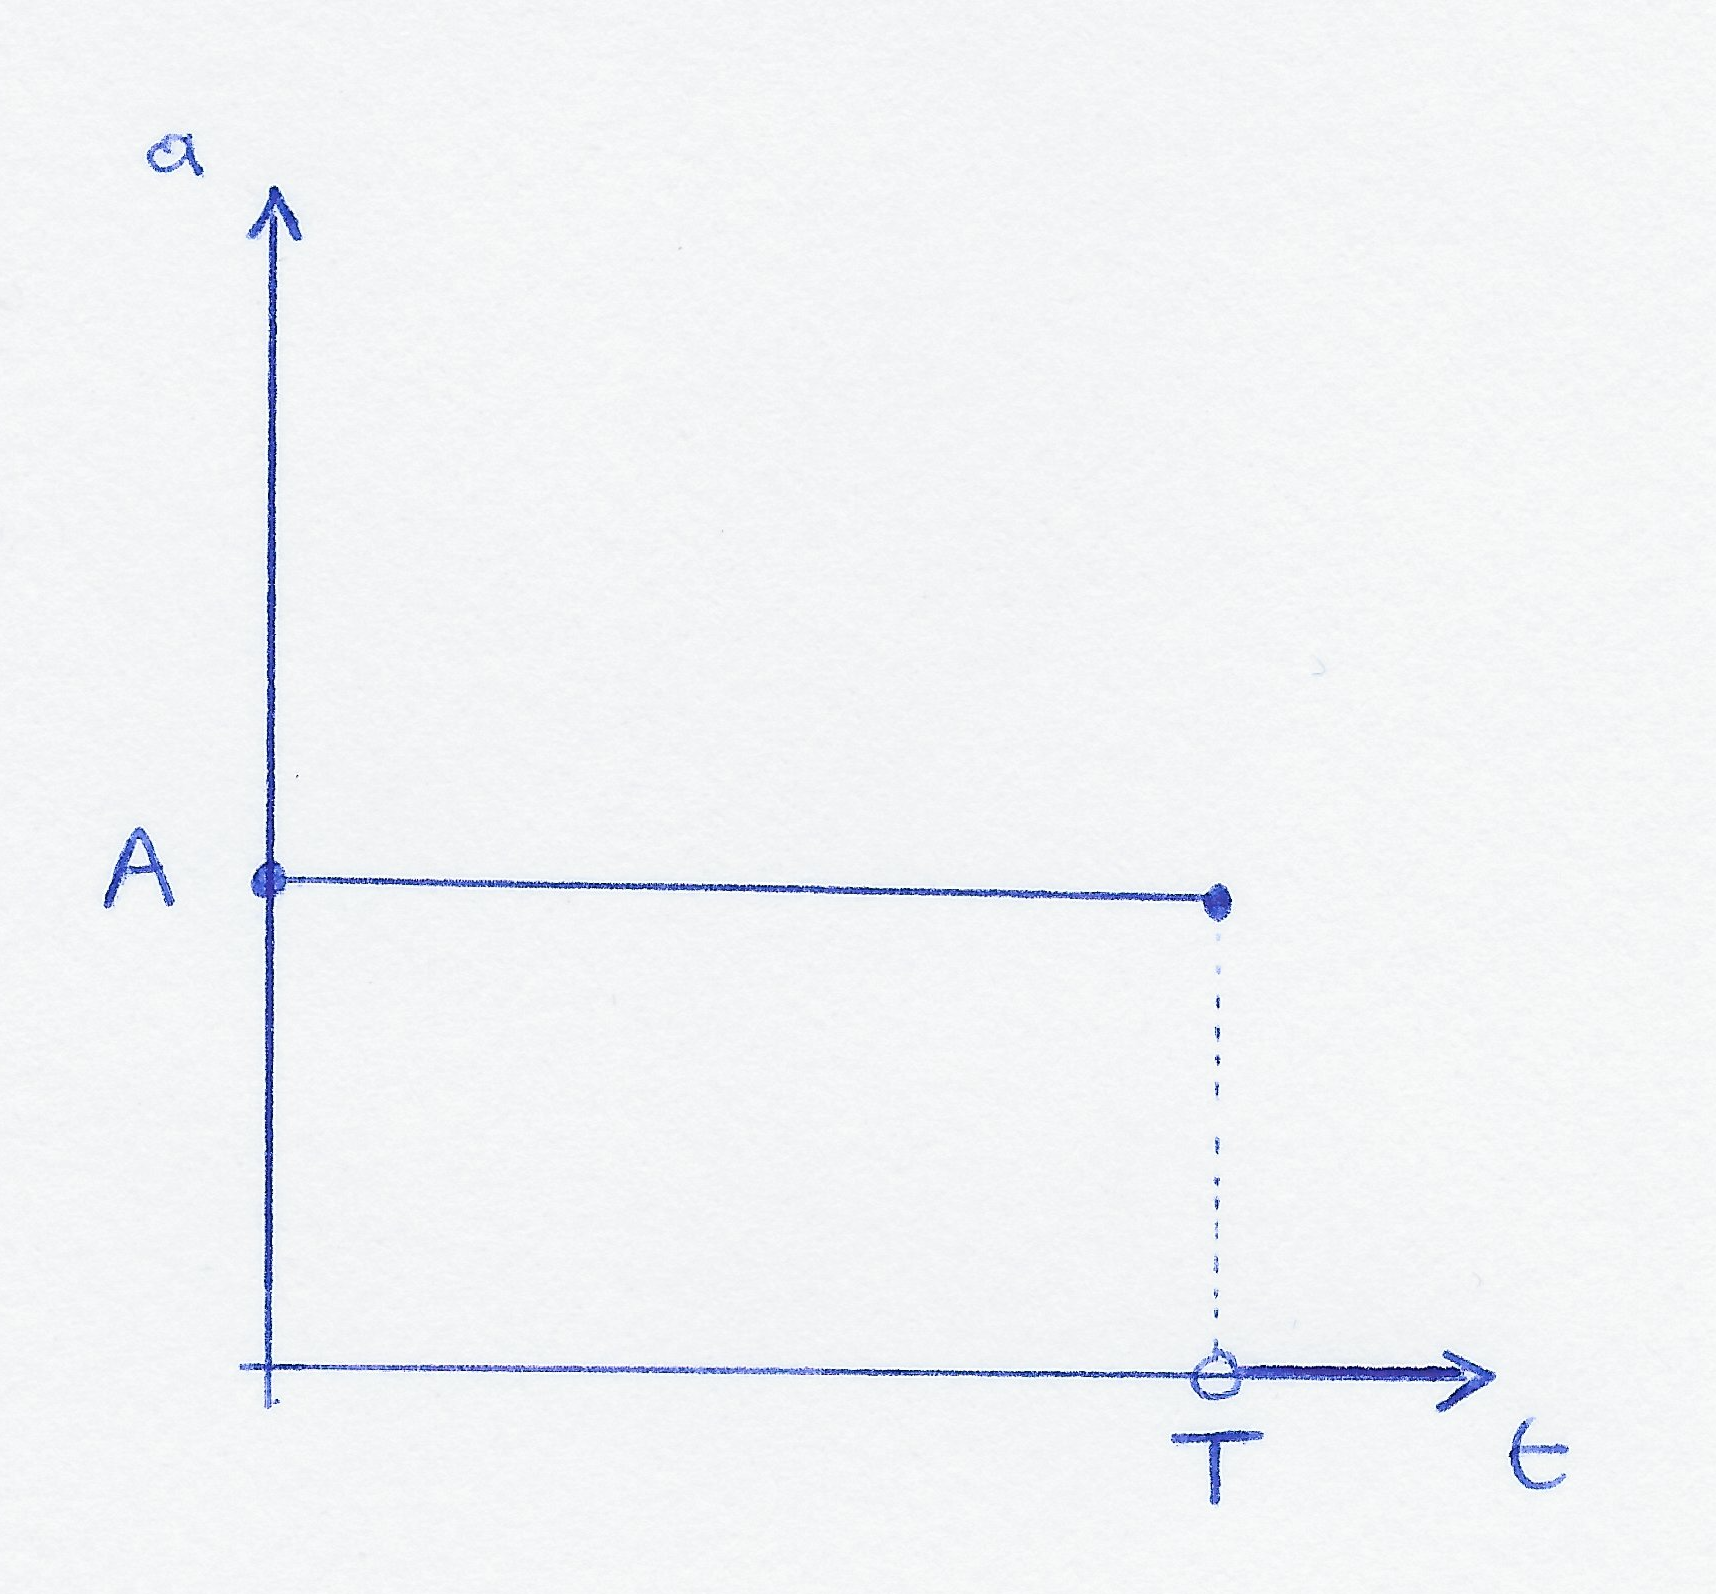
\includegraphics[scale=0.07]{figures/uniform-acc}
\caption{Profile of uniform acceleration}
\end{figure}
\end{frame}

%------------------------------------------------

\begin{frame}
\frametitle{Control}
\framesubtitle{Speed control(2/5)}
For a smoother transition (based on instinct) the robot accelerates following the profile as Fig.\ref{fig:smooth-acc}. However, we want the robot to acheive the target speed in the same amount of time as uniform. This is translated in eq ref.
\begin{columns}[c]

\column{.35\textwidth}
\begin{align*}
&\Leftrightarrow \int_{0}^{T}a(t) =  \int_{0}^{T}a'(t) \\
&\Leftrightarrow A\,T = \underbrace{d\,B}_{triangles} + \underbrace{(T - 2d)B}_{rectangle}
\end{align*}

\column{.55\textwidth}
\begin{figure}[hbtp]
\centering
\label{fig:smooth-acc}
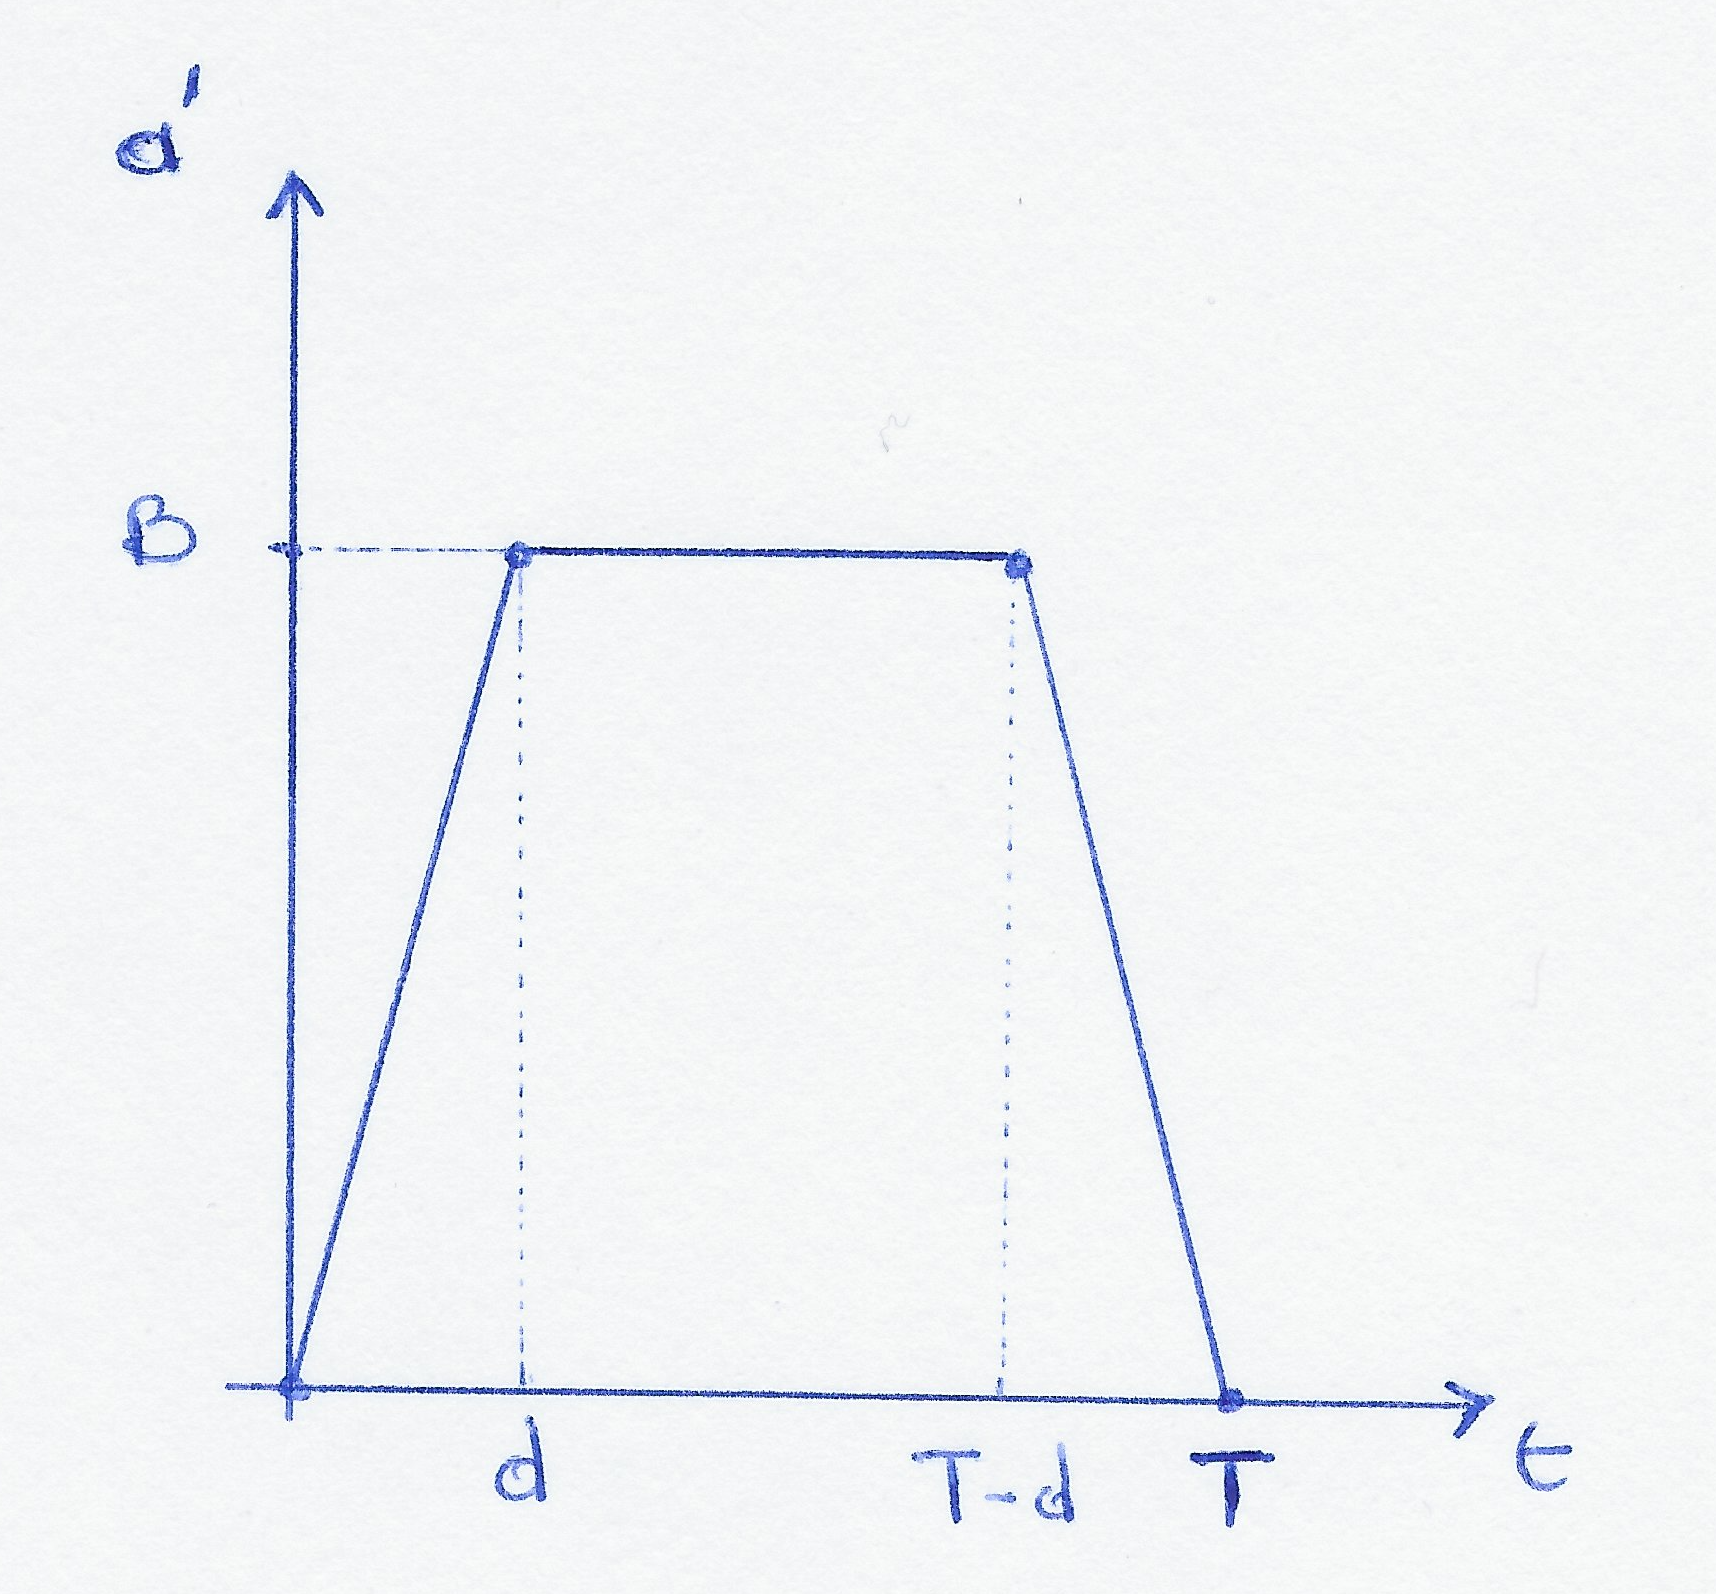
\includegraphics[scale=0.07]{figures/smooth-acc}
\caption{Profile of smooth acceleration}
\end{figure}
\end{columns}
\end{frame}

%------------------------------------------------

\begin{frame}
\frametitle{Control}
\framesubtitle{Speed control (3/5)}
By introducing the parameter $\psi = \frac{d}{T}$, equation ref can be rewritten as
$$
\boxed{B = \frac{A}{1-\psi}} 
$$
The update rule for the progress speed becomes
$$
v_{n+1} \leftarrow v_n + \int_{n}^{n+1}a'(t) = v_n + \int_{0}^{n+1}a'(t) - \int_{0}^{n}a'(t)
$$
Note that splitting the integrals permits us to simplify calculations by making use of fixed surfaces.
\end{frame}

%------------------------------------------------

\begin{frame}
\frametitle{Control}
\framesubtitle{Speed control (4/5)}
\begin{figure}[hbtp]
\centering
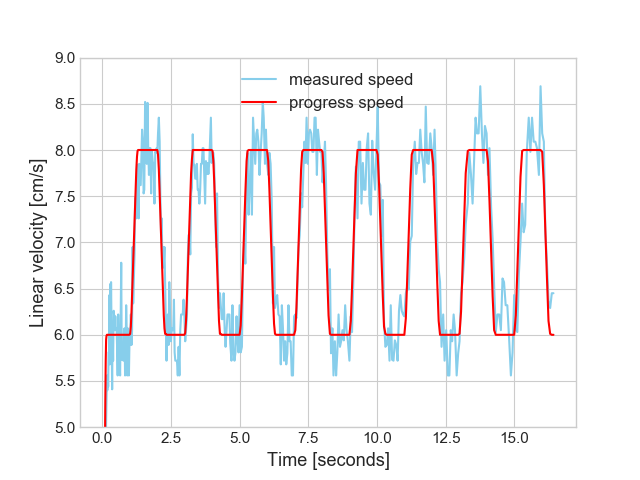
\includegraphics[scale=0.45]{figures/pid_speed_normal.png}
\caption{Full view}
\end{figure}
\end{frame}

%------------------------------------------------

\begin{frame}
\frametitle{Control}
\framesubtitle{Speed control (5:5)}
\begin{figure}[hbtp]
\centering
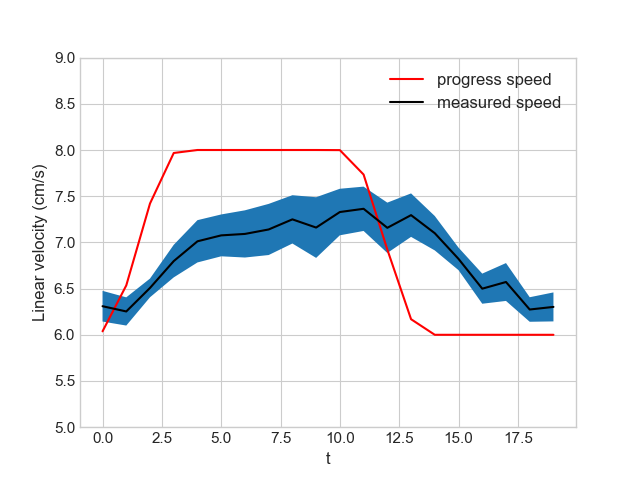
\includegraphics[scale=0.45]{figures/pid_speed_shaded.png}
\caption{+- 2 standard error with mean}
\end{figure}
\end{frame}

%------------------------------------------------

\begin{frame}
\frametitle{Control}
\framesubtitle{Turning (1/2)}
We model the COEX-1 as a two-wheel robot as in Fig.\ref{fig:model-turn}. By integrating the angular velocity under the assumption that $v_R = -v_L$, we obtain 
$$
\theta(t) = \frac{2vt}{b} + \theta_0
$$
\begin{figure}[hbtp]
\centering
\label{fig:model-turn}
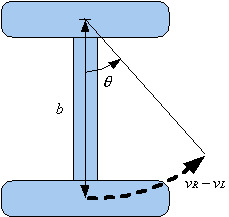
\includegraphics[scale=0.45]{figures/differential-system.jpg}
\caption{Two wheel model}
\end{figure}
\end{frame}

%------------------------------------------------

\begin{frame}
\frametitle{Control}
\framesubtitle{Turning (2/2)}
Based on equation ref, we can make the robot turn $\Theta$ radians as follows:
\begin{algorithmic}[1]
\State $\theta\gets 0$
\State \Call{Turn}{$v_{target}$}
\While{$\theta < \Theta$}
\State $\theta_{n+1} \gets \frac{2\, v_n\, \Delta_{n:n+1}}{b}$
\EndWhile
\State \Call{StopMotors}{}
\end{algorithmic}
Some error because not pure rotation, noise etc. Error seems reasonable 5 to 10 degrees. However not good enough for robust turning when exploring environment. Other method developped in section ref.
\end{frame}


%------------------------------------------------
\section{Exploration \& Mapping} 
%------------------------------------------------

\begin{frame}
\frametitle{Overview}
\tableofcontents[currentsection,subsectionstyle=shaded]
\end{frame}

%------------------------------------------------
\begin{frame}
\frametitle{Exploration \& Mapping}
\framesubtitle{General}
To explore an unknown environment structured as a maze it needs to be able to:
\begin{itemize}
\item Compute the distance travelled since the last intersection (slide ref)
\item Detect an intersection (slide ref)
\item Turn to the desired intersection (slide ref)
\end{itemize}
\end{frame}

%------------------------------------------------

\begin{frame}
\frametitle{Exploration \& Mapping}
\framesubtitle{Distance (1/5)}
First method: Simple equation - explain without mathematics.\\~\\
Second method: Upperbound of error can be reduced due to relation with distance.\\~\\
plot relationship
\end{frame}

%------------------------------------------------

\begin{frame}
\frametitle{Exploration \& Mapping}
\framesubtitle{Distance (2/5)}
Plot comparison with error bars of two methods on test set.\\~\\
Conclusion.
\end{frame}

%------------------------------------------------

\begin{frame}
\frametitle{Exploration \& Mapping}
\framesubtitle{Distance (3/5)}
Explain we could try to quantify uncertainty and above certain threshold not accept it.\\~\\
$$
	MSE = \sum_{i=0}^N err_{line}^2
$$
obtained iteratively by rolling mean method.
One plot 
\end{frame}

%------------------------------------------------

\begin{frame}
\frametitle{Exploration \& Mapping}
\framesubtitle{Distance (4/5)}
Explain simpler choice is to discretize from second method discretization.\\~\\
Remard 7.5-12.5 ....\\~\\
Plot discretization on test set.
\end{frame}

%------------------------------------------------

\begin{frame}
\frametitle{Exploration \& Mapping}
\framesubtitle{Distance (5/5)}
Example of resulting big map. Explain annotation\\~\\
Map.
\end{frame}

%------------------------------------------------

\begin{frame}
\frametitle{Exploration \& Mapping}
\framesubtitle{Intersection detection}
Approach developped to intersection detection is based on majority vote idea. $x_{loc}$ takes value 1 if a black line is detected at location loc. From moment anomalie detected we start following procedure.
$$
y_{loc} = \underset{x \in  \{0,1\}}{\operatorname{argmax}} \operatorname{mode}(x_{loc})
$$
Boolean value for intersection based on decision rule as follows
$$
(y_{center} = 0) \lor (y_{left} = 1) \lor (y_{right} = 1) 
$$
\end{frame}

%------------------------------------------------

\begin{frame}
\frametitle{Exploration \& Mapping}
\framesubtitle{Intersection classification}
We use the values computed during intersection detection, and we make the robot go a bit further forward. The type of intersection is determined and takes values in following set:
\begin{figure}[hbtp]
\centering
\label{fig:type-intersection}
\includegraphics[scale=0.06]{figures/type-intersection}
\caption{The 7 types of intersections}
\end{figure}
\end{frame}

%------------------------------------------------

\begin{frame}
\frametitle{Exploration \& Mapping}
\framesubtitle{Turning \& alignment (1/2)}
Problem with naive approach.\\~\\
Solution + plot + equation.
\end{frame}

%------------------------------------------------

\begin{frame}
\frametitle{Exploration \& Mapping}
\framesubtitle{Turning \& alignment (2/2)}
Explain plot.\\~\\
Plot to verify results.\\~\\
Explain why not such a good idea.
\end{frame}

%------------------------------------------------
\section{Code} 
%------------------------------------------------

\begin{frame}
\frametitle{Overview}
\tableofcontents[currentsection,subsectionstyle=shaded]
\end{frame}

%------------------------------------------------
\begin{frame}
\frametitle{Code}
\framesubtitle{General architecture}
\begin{figure}[hbtp]
\centering
\label{fig:architecture}
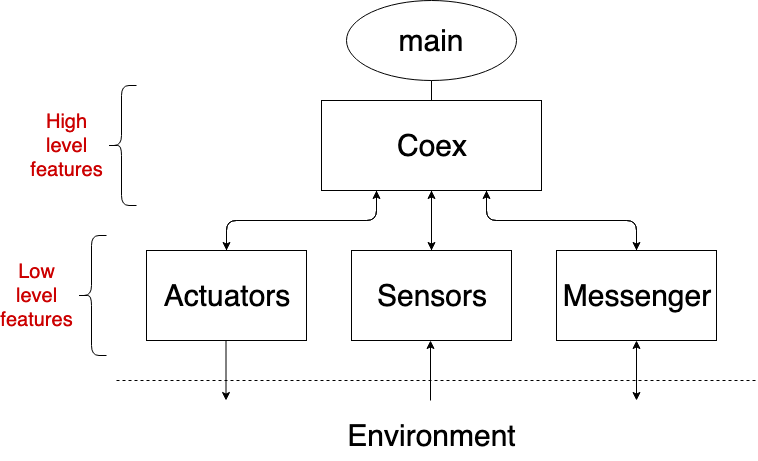
\includegraphics[scale=0.38]{figures/architecture.png}
\caption{Architecture of the code}
\end{figure}
\end{frame}


%------------------------------------------------

\begin{frame}
\begin{figure}[hbtp]
\centering
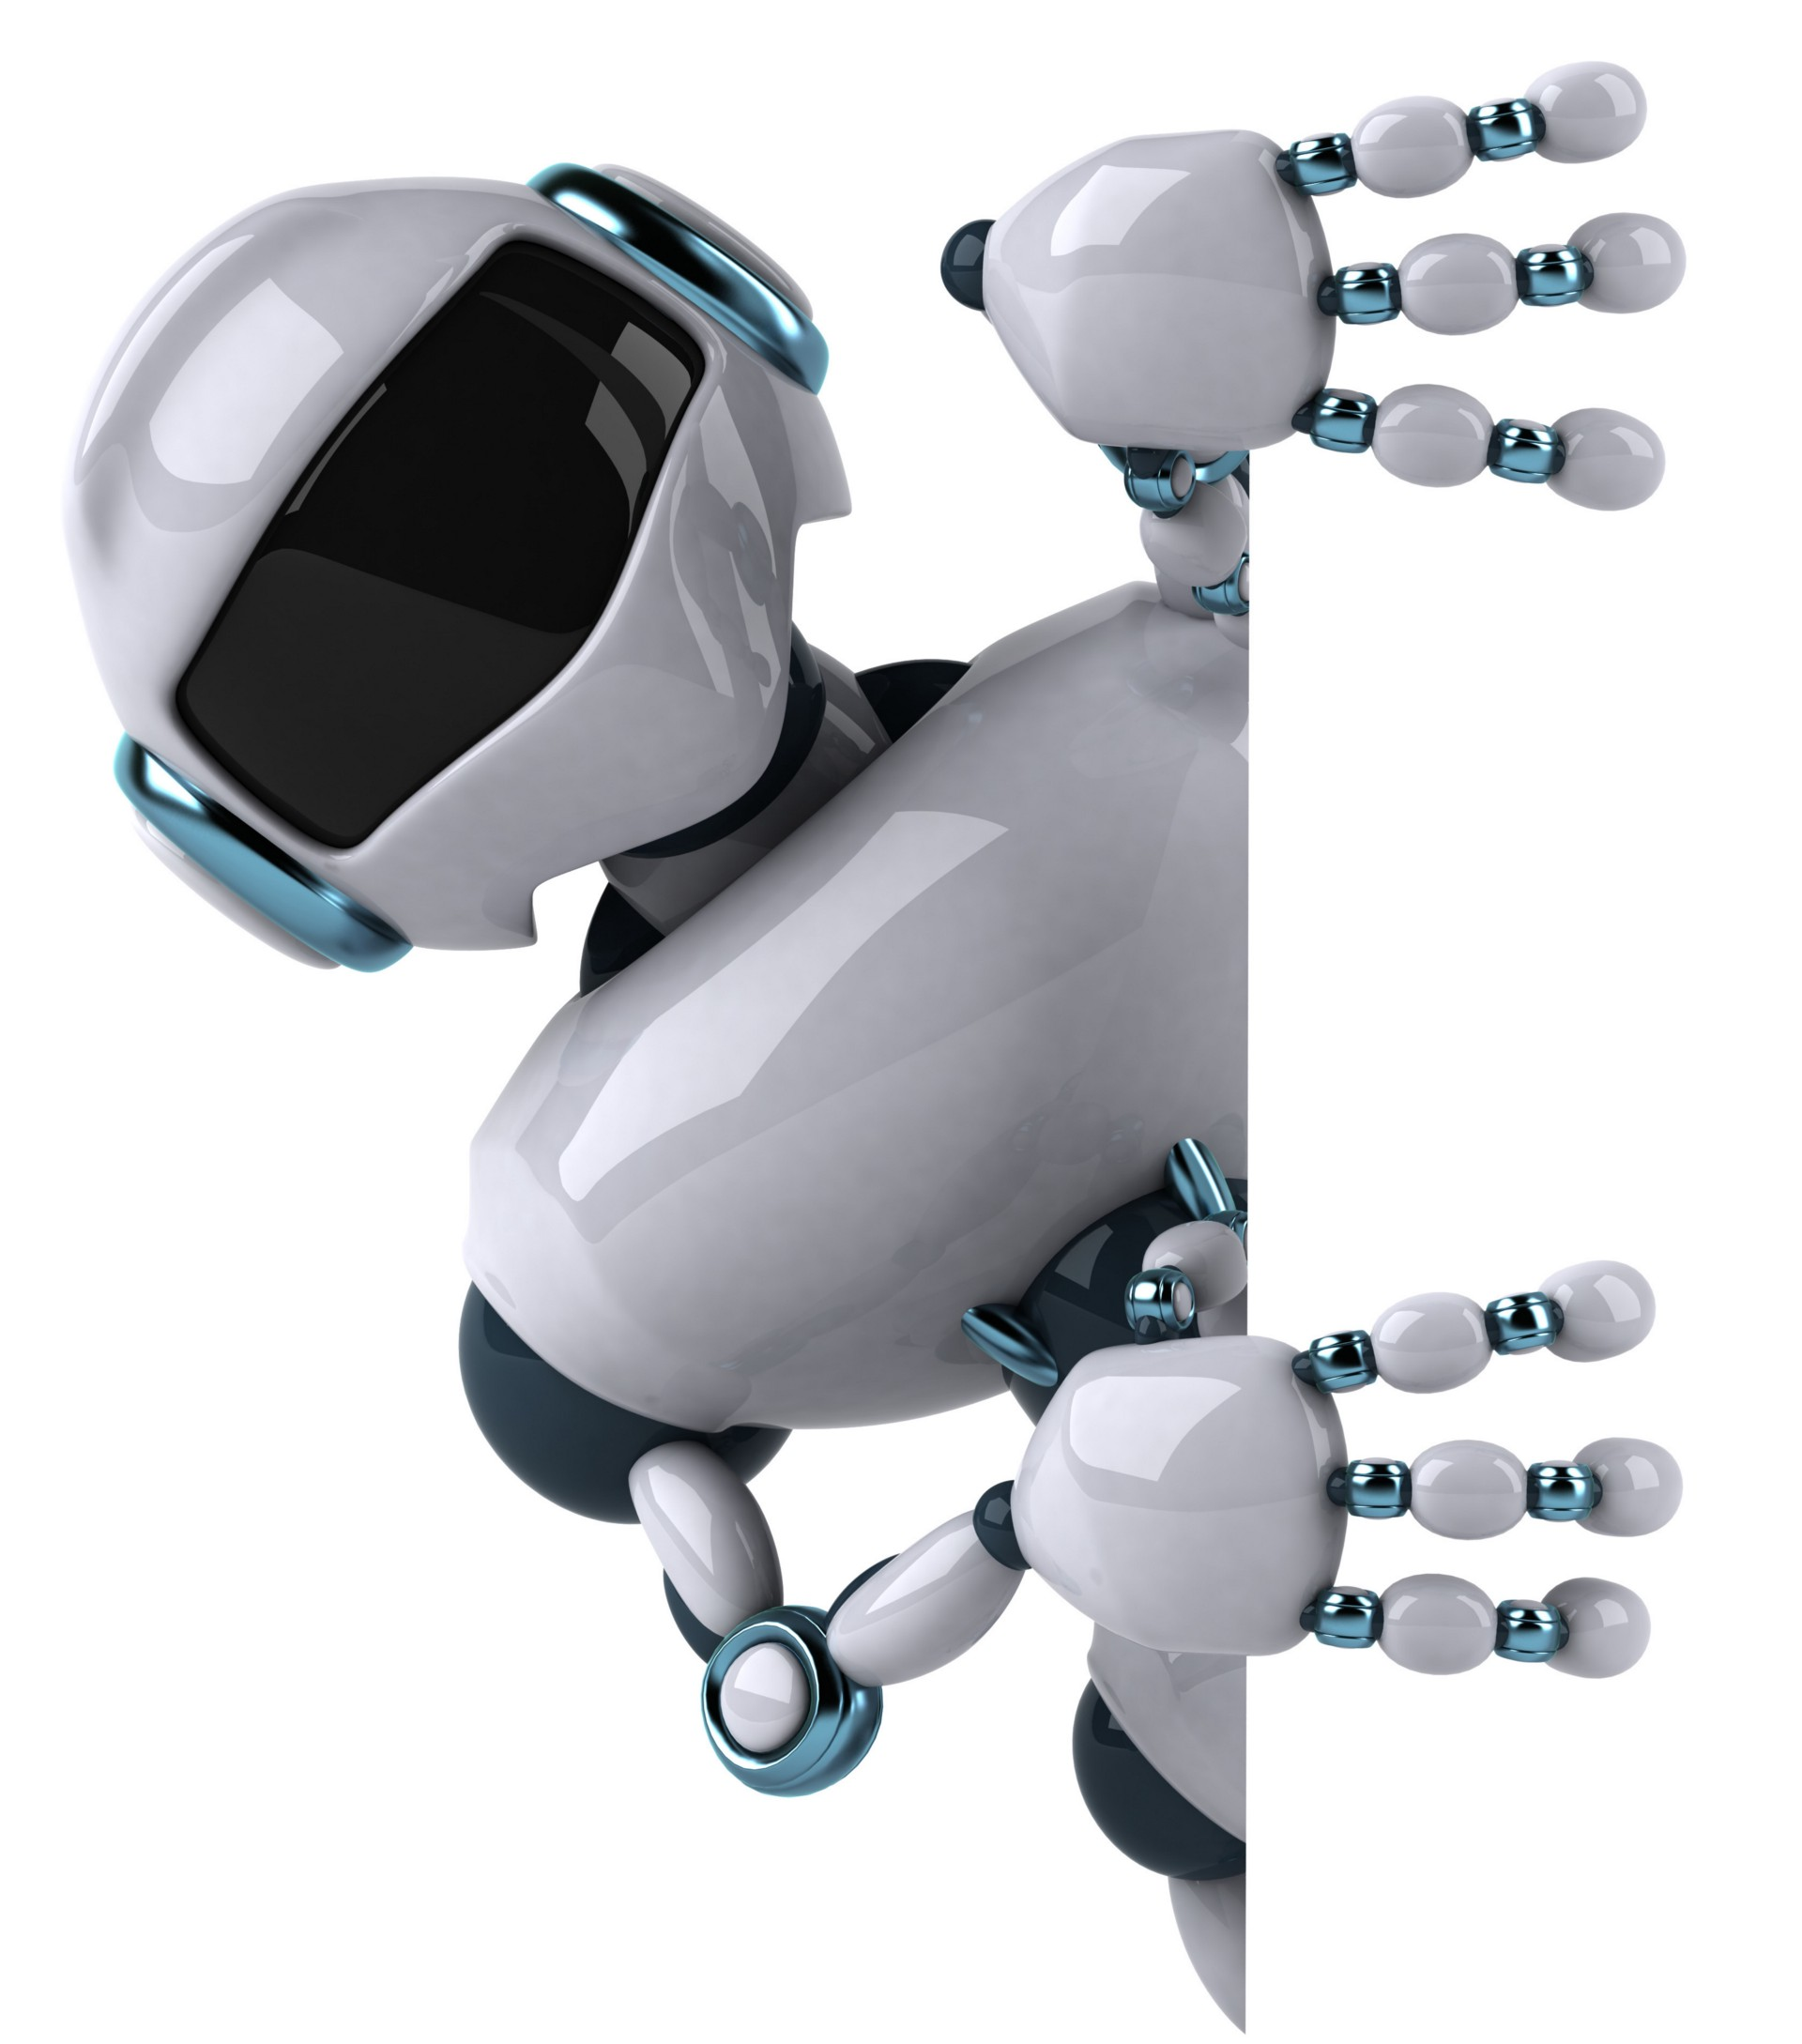
\includegraphics[scale=0.1]{figures/bye-bye.jpeg}
\end{figure}
\end{frame}

%----------------------------------------------------------------------------------------

\end{document}
